\chapter{Hintergrund}


\section{Scikit-learn}
Scikit-learn (\cite{scikit-learn}) ist die Software-Bibliothek welche für das Implementieren der verschiedenen Klassifikationsalgorithmen genutzt wurde. Es handelt sich hierbei um eine freie Software-Bibliothek zum maschinellen Lernen für die Programmiersprache Python.
 

\section{Muskel}
Muskeln können in drei Typen unterteilt werden: quergestreifte, Herz- und glatte Muskeln. Die beiden letzteren sind für diese Arbeit nicht von Interesse, da nur Gesichtsmuskeln, bei denen es sich um quergestreifte Muskeln handelt, beobachtet werden. Quergestreifte Muskulatur bildet die Skelettmuskulatur   (\ref{fig:uka1}). Als Skelettmuskeln bezeichnet man diejenigen Muskeln, die  für die  Körperbewegungen zuständig sind. \cite{trainingsworld}

Der Aufbau eines Muskels  ist eine Spindel ähnliche Form, die im oberen und unteren Bereich dünner wird.  
Der Muskel besteht aus Muskelfaserbündeln, welche wiederum aus vielen Muskelfasern bestehen. Die Muskelfasern bestehen aus Myofibrillen.
Die Myofibrillen bestehen abermals aus Filamenten, welche sich in zwei verschiedene Typen aufteilen lassen. Diese Filamente sind die Myosinfilamente und die Aktinfilamente. Der Aufbau ist in der Abbildung \ref{fig:muskel1} zu sehen. 

\begin{figure}[H]
  \centering
  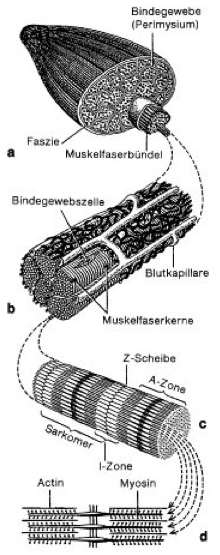
\includegraphics[width=70mm,height=10cm,scale=0.6]{MuskelAufbau.png}
  \caption{Aufbau eines Muskels \cite{Spektrum}}
  \label{fig:muskel1}
\end{figure}

\subsection{Motorische Einheit}

Eine Motorische Einheit \cite{MorSteMer2004-ATO} besteht aus einer Nervenzelle, einer Nervenfaser und einer Muskelfasern. Die Motorische Einheit ist für die Kontraktion der Muskeln durch Nervenimpulse zuständig. Dabei steuert jede motorische Nervenzelle jeweils mehrere Muskelfasern \ref{fig:muskel2}. Bei diesen Nervenimpulsen handelt es sich um die im Weiteren erklärten Aktionspotenziale.

\begin{figure}[H]
  \centering
  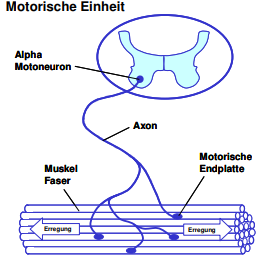
\includegraphics[width=70mm,scale=0.7]{MotorUnit.png}
  \caption{Aufbau einer Motorischen Einheit  \cite{KonEMG2006-ATO}}
  \label{fig:muskel2}
\end{figure}

\clearpage

\subsection{Muskelkontraktion}
Muskelkontraktionen sind notwendig für die menschliche Bewegung. 
Eine Muskelkontraktion \cite{MorSteMer2004-ATO} wird durch das Bilden einer ionischen Differenz zwischen dem Innen- und Außenraum einer Muskelzelle ausgelöst. Der Konzentrationsunterschied zwischen dem Inneren und Äußeren der Muskelzelle verursacht ein 
Ruhepotenzial.
Diese Potenzialdifferenz wird durch eine Ionenpumpe aufrechterhalten. Über das Axon kommt ein Reiz von der Motorischen Einheit an die motorische Endplatte (Verbindung zwischen den Synapsen) und der Muskelfaser. Wenn es zu einem Reiz kommt, kommt es zu einem Na+ Einstrom und einem K+ Ausstrom. Dies bewirkt eine Depolarisation, die sofort durch rückwärts Austausch von Ionen durch die Ionenpumpen umgekehrt wird
(Repolarisation). In \ref{fig:AP3} ist die Muskelkontraktion aus einer chemischen Perspektive zu sehen.


\begin{figure}[H]
  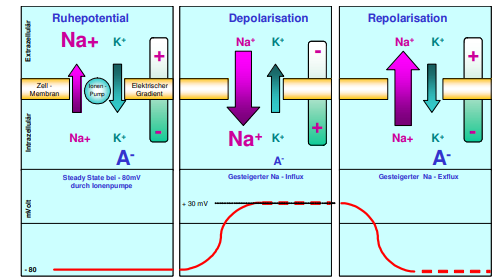
\includegraphics[width= \linewidth]
{Aktionspotenzial3.png}
  \caption{Das Aktionspotenzial aus der Perspektive der Ionen \cite{KonEMG2006-ATO}}
  \label{fig:AP3}
\end{figure}


\subsubsection{Potenzialverlauf}
Aktionspotenziale können in vier Phasen eingeteilt werden  (siehe \ref{fig:AP3}):


1. In der Anfangsphase treibt ein Reiz die negative Spannung in Richtung null.

2. Beim Überschreiten einer bestimmten Na+ Konzentration, beschleunigt sich die Depolarisation sehr stark. Das führt dazu, dass die Membranpotenzial sehr schnell von positiv zu negativ wechselt. 

3. Nach dem Erreichen des Maximums bewegt sich das Aktionspotenzial zum Anfangswert, also dem Ruhepotenzial, zurück.

4. Das Ruhepotenzial wird unterschritten(Hyperpolarisation) und schließlich wieder erreicht. \cite{KonEMG2006-ATO}

\begin{figure}[H]
  \centering
  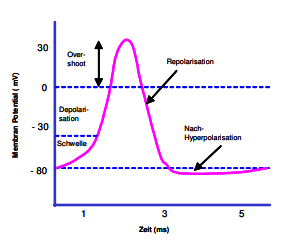
\includegraphics[width=120mm,scale=0.7]{Aktionspotenzial.png}
  \caption{Verlauf des  Aktionspotenzials in den verschiedenen Phasen \cite{KonEMG2006-ATO}}
  \label{fig:AP1}
\end{figure}


\section{Sprachproduktion}

\subsection{Relevante Muskeln}
In diesem Teil werden die relevanten Muskeln für die Sprachbildung aufgelistet. Die Informationen in diesem Teil kommen aus der Diplomarbeit von Matthias Janke \cite{janke2016emg}. Die Positionen der Muskeln im Gesicht sind in der Abbildung \ref{fig:FaceMusc} zu sehen.

\paragraph{Zunge}
Die Zunge  ist eine Verbindung aus intrinsischen und extrinsischen Muskeln. Sie nimmt den größten Teil der Mundhöhle ein und hat damit großen Einfluss
auf die Vokalartikulation. Die Vokale sind durch die Position der Zunge charakterisiert. Es werden keine Daten der Zunge für diese Arbeit genutzt.

\paragraph{Orbicularis oris} 
Orbicularis oris ist ein runder Muskel. Dieser zieht sich zusammen, um die Lippen zu bewegen.
\paragraph{Levator labii superioris}
Levator labii superioris zieht die Oberlippe nach oben.
\paragraph{Zygomaticus major und minor}
Zygomaticus major und minor ziehen die Mundwinkel nach oben und nach hinten zurück, beim Lächeln zum Beispiel.
\paragraph{Depressor anguli oris}
Der Depressor anguli oris zieht die Mundwinkel nach unten.
\paragraph{Depressor labii inferioris}
Depressor labii inferioris senkt die Unterlippe ab.
\paragraph{Risorius}
Risorius zieht die Lippenecken zurück.
\paragraph{Mentalis}
Mentalis zieht die Unterlippe nach vorne und ihre Kontraktion führt zu einer Vorwölbung der Lippenwinkel und zum Bewegen der Unterlippe.
\paragraph{Buccinator}
Buccinator komprimiert die Kontrolle und zieht den Mundwinkel zurück.
\paragraph{Platysma}
Platysma ein großer Muskel, der unter dem Kiefer und im Nacken bis zur oberen Brust reicht. Dieser Muskel drückt auf den Unterkiefer und hilft dabei, die Lippen zu senken.
\paragraph{Masseter}
Der Masseter ist ein kräftiger Muskel, der den Kiefer schließt. Der Masseter Muskel ist in der Abbildung leider nicht zu sehen. Es handelt sich dabei um den Kaumuskel.

\begin{figure}[H]
  \centering
  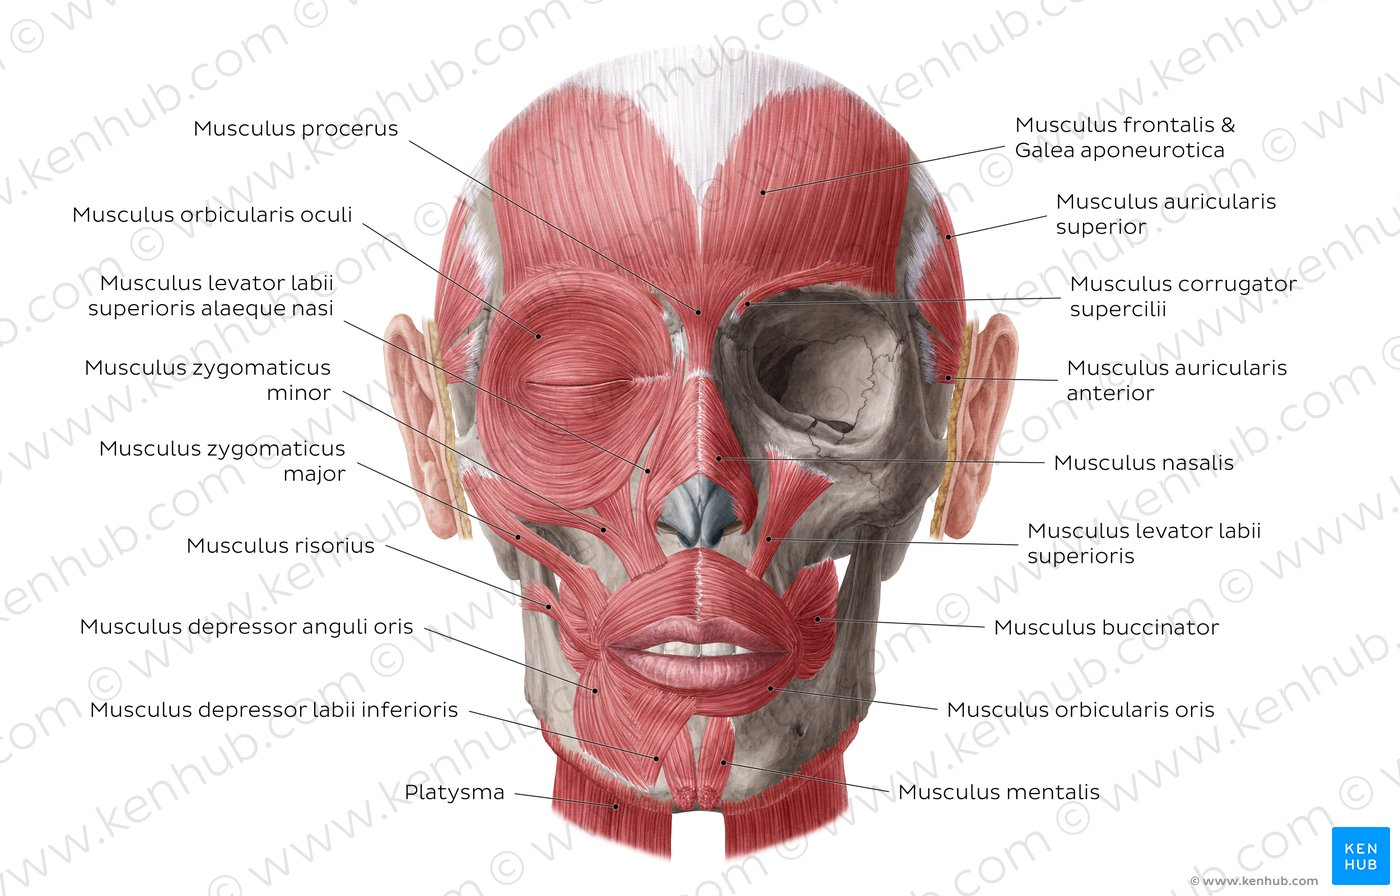
\includegraphics[width=\linewidth]{FaceMuscle.png}
  \caption{Die Muskeln im Gesicht eines Menschen.  \cite{kenhub}}
  \label{fig:FaceMusc}
\end{figure}


\subsection{Mechanismus}
Abbildung \ref{fig:sp1} zeigt den Querschnitt der Anatomie des Sprachsystems innerhalb des menschlichen Oberkörpers. Die groben Komponenten des Systems sind die Lunge, die Luftröhre, der Kehlkopf, der Rachenraum, der Mund und die Nase. Die Rachen- und Mundhöhle können zu einer Einheit, die als Vokaltrakt bezeichnet wird, zusammengefasst werden und die Nasenhöhle wird oft als Nasaltrakt bezeichnet.
Weitere für die Sprachproduktion entscheidende Organe, sind die Stimmbänder, die Lippen, die Zunge, die Zähne und das Velum.
Der Unterkiefer ist sowohl für grobe als auch feine Bewegungen verantwortlich, welche die Größe und Form des Vokaltrakts sowie die Positionen der anderen Artikulatoren beeinflussen. \cite{Docio-Fernandez2015}

Der Nasaltrakt, Rachenraum und der Mund sind wichtig für die Sprachproduktion. In der Arbeit von Matthias Janke \cite{janke2016emg} wird die Sprachentwicklung nach der Reihenfolge des Luftstroms erklärt. Dabei wird von Anfang des Luftstroms in der Lunge bis zum Ende des Luftstroms im Nasaltrakt unterschieden. Dabei ist die Lunge die Quelle für die Luft. Die Luft strömt in den Kehlkopf zu den Stimmbändern, von da aus in den Rachen. Danach weicht ein Teil der Luft aus dem Mund hinaus, woraus sich die gesprochene Sprache ergibt. Der Rest der Luft verlässt den Körper durch die Nase. Die Position des Kehlkopfs und Rachen ist in \ref{fig:sp1111} zu sehen.


\begin{figure}[H]
  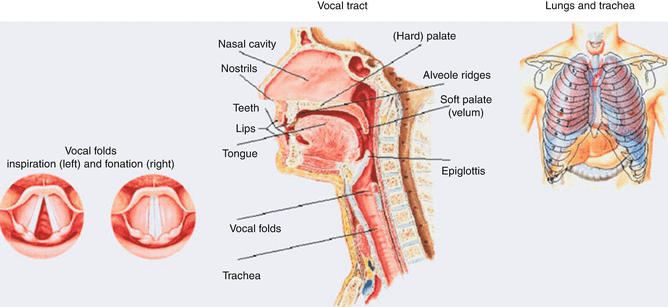
\includegraphics[width=130mm,scale=1]{humanSpeech.png}
  \caption{Die Einzelteile der Menschlichen Sprachproduktion \cite{Docio-Fernandez2015} }
  \label{fig:sp1}
\end{figure}

\begin{figure}[H]
  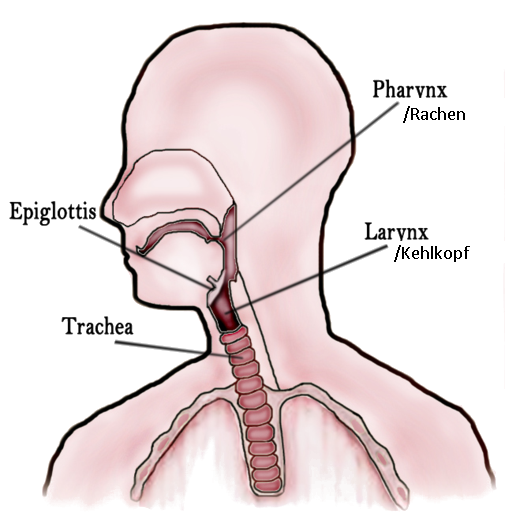
\includegraphics[width=80mm,scale=1]{ThroatDiagram.png}
  \caption{Positionen des Pharynx und Larynx. \cite{Wikimedia-Common4}}
  \label{fig:sp1111}
\end{figure}
  


\section{EMG}
In der Elektromyografie (EMG) geht es um das Messen der Muskelfunktion durch die Aufzeichnung des elektrischen Signals, welches vom relevanten Muskel stammt. Diese elektrischen Signale beziehen sich auf die zuvor beschriebenen Aktionspotenziale. 

Es wird zwischen zwei Arten von EMG unterschieden, der intramuskulären EMG und der Oberflächen-EMG.
In der intramuskulären EMG werden Nadelelektroden durch die Haut in das Muskelgewebe eingeführt. Dies ist nützlich, wenn man Aktionspotenziale einzelner Muskelfasern messen will. Zum Beispiel um durch das EMG-Signalmuster Muskelkrankheiten zu erkennen.
Oberflächen-EMG ist hingegen die Aufzeichnung von Signalen mit Hilfe von auf der Haut angebrachten Oberflächenelektroden, es ist also im Vergleich zur intramuskulären EMG nicht invasiv. Oberflächenelektroden haben zudem den Nachteil, dass nur
oberflächliche Muskeln abgeleitet werden können.   \cite{KonEMG2006-ATO}.

\subsection{Digitalisierung}
In \ref{fig:REMG} ist ein rohes EMG-Signal zu sehen. Die Grundlinie ist das vordefinierte Grundlinienrauschen. Die drei Kontraktionssalven stammen aus drei Kontraktionen des Bizeps. Das EMG-Signal hat eine stochastische Natur, ist also nicht in ihrer exakten Form reproduzierbar. Dieses Rohsignal wird dann vom Analogen ins Digitale umgewandelt. In \ref{fig:DEMG} kann man sehen was für einen Einfluss das Wählen der Abtastrate auf die Digitalisierung des Rohsignals hat. Zudem sieht man das Ergebnis der Digitalisierung mit verschiedenen Abtastfrequenzen. \cite{KonEMG2006-ATO}

\begin{figure}[H]
  \centering
  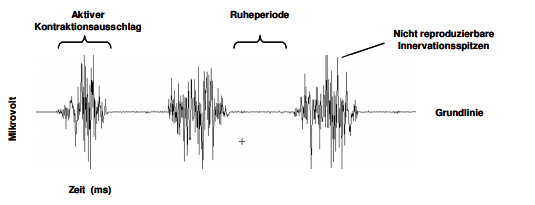
\includegraphics[width= \linewidth]{RohEMG.png}
  \caption{Die Roh-EMG-Signalaufzeichnung dreier Kontraktionssalven.  \cite{KonEMG2001-ATO}}
  \label{fig:REMG}
\end{figure}

\begin{figure}[H]
  \centering
  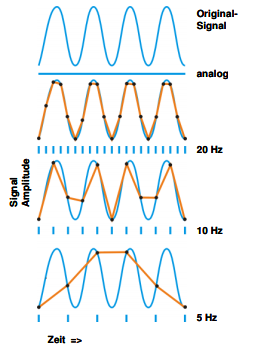
\includegraphics[width= 100mm]{DigEMG.png}
  \caption{ Der Einfluss der A/D-Abtastfrequenz auf das digitalisierte Signal.  \cite{KonEMG2001-ATO}}
  \label{fig:DEMG}
\end{figure}

\section{Datenkorpus}
Der Datensatz, den ich für diese Arbeit verwendet habe, ist der \cite{WaJaSch2014-IS} UKA-Korpus des CSL in Bremen. Hierbei handelt es sich um eine Sammlung von Oberflächen EMG Aufnahmen von verschiedenen Sprechern in verschiedenen Sprachmodi. Kanal 5 wurde in dieser Arbeit nicht entfernt. 


Die Elektrodenpositionen für die Aufnahmen, sowie die relevanten Muskeln sind in der Figur  \ref{fig:uka1} zu sehen. 
Die EMG-Daten wurden mit einer Sechskanal-Elektrodenanordnung aufgezeichnet. \ref{fig:uka1} zeigt die Positionierung der Elektroden, die das EMG-Signal von sechs artikulatorischen Muskeln aufzeichnen. Eine zusätzliche Erdelektrode wurde am Handgelenk der Probanden platziert. \cite{WaJaSch2014-IS}. 

\begin{figure}[H]
  \centering
  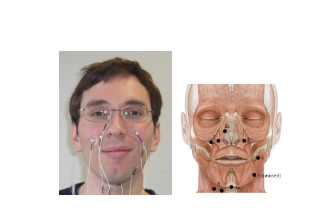
\includegraphics[width=80mm]{UKARecording.png}
  \caption{Elektrodenpositionierung für den EMG-UKA Korpus  \cite{WaJaSch2014-IS}}
  \label{fig:uka1}
\end{figure}

\subsection{Informationen zu den Daten}
Die Daten wurden in große Sessions, Multi-Mode-Sessions und kleine Sessions aufgeteilt \ref{fig:uka3}. Die Multi-Mode Sessions sind für die Bestimmung des Sprachmodus relevant, denn diese liefern 50 Aufnahmen für jeden Sprachmodus. Die großen Sessions beinhalten mehr als 500 Aufnahmen für den hörbaren Modus. Für die Aufteilung der Sessions nach Sprachmodi sowie die Anzahl der Sessions, durchschnittliche Länge und gesamte Länge der Sessions siehe \ref{tab:uka2}. Die großen Sessions wurden in der Sprachmodus Erkennung  nicht verwendet, da sie nur aus hörbaren Aufnahmen bestehen \cite{WaJaSch2014-IS}. 

\begin{table}[H]
 \centering
 \caption{Datenmenge im EMG-UKA-Korpus. \cite{WaJaSch2014-IS}}
\begin{tabular}{|c|cccc|}
\hline 
 & \multicolumn{3}{c}{Anzahl der Sessions} &\\ 
\hline 
 Sprecher& Gesamt & Groß & Multi-Mode & \\ 
\hline 
1 & 3 & 0 & 3 &\\ 
\hline 
2 & 33 & 1 & 15 & \\ 
\hline 
3 & 1 & 0 & 1 &\\ 
\hline 
4 & 2 & 0 & 2 &\\ 
\hline 
5 & 1 & 0 & 1 & \\ 
\hline 
6 & 1 & 0 & 1 & \\ 
\hline 
7 & 2 & 0 & 2 & \\ 
\hline 
8 & 20 & 1 & 7 & \\ 
\hline 
Gesamt & 63 & 2 & 32 & \\ 
\hline   
\label{tab:uka2} 
\end{tabular} 
\end{table}

\begin{table}[H]
 \centering
\caption{Zusammenfassung der Sitzungen im gesamten EMG-UKA-Korpus.\cite{WaJaSch2014-IS} }
\begin{tabular}{|c|c|c|c|c|}
\hline 
Teilmenge & \#Sprecher & \#Sessions & Durchschnitt & Gesamt \\ 
\hline 
Hörbar(Klein) & 8 & 61 & 3:08 & 3:11:34 \\ 
\hline 
Flüsternd(Klein) & 8 & 32 & 3:22 & 1:42:42 \\ 
\hline 
Stumm(Klein) & 8 & 32 & 3:19 & 1:46:20 \\ 
\hline 
Hörbar(Groß) & 2 & 2 & 27:02 & 54:04 \\ 
\hline 
\multicolumn{5}{|c|}{Gesamt Menge an Daten ist 7:32 Stunden} \\ 
\hline
  \label{fig:uka3} 
\end{tabular} 
\end{table}



\subsection{Sprachmodus}
Der Sprachmodus wird in dieser Arbeit in drei verschiedene Modi aufgeteilt. Die Sprecher wurden angewiesen, alle Sprachmodi so zu produzieren, wie sie sich am natürlichsten anfühlen \cite{WaJaSch2014-IS}. Die englischen sowie die deutschen Namen für die verschiedenen Sprachmodi, wurden in dieser Arbeit verwendet.

\paragraph{Hörbare Sprache(Audible Speech)}
Bei der hörbaren Sprache handelt es sich um die normale Stimme die von den Sprechern benutzt wird.   

\paragraph{Geflüsterte Sprache (Whispered Speech)}
Geflüsterte Sprache wird erzeugt, wenn die Stimmbänder nicht vibrieren, sondern zusammengezogen werden.  Dies führt dazu, dass die normale Grundfrequenz des Sprechers durch einen zischenden Ton ersetzt wird. Im EMG-UKA-Korpus werden hörbare und geflüsterte Sprache als getrennte Sprachmodi betrachtet, obwohl geflüsterte Sprache auch hörbar ist.

\paragraph{Stumme Sprache (Silent Speech)}
Stumme Sprache bedeutet, dass der Sprecher zwar normale artikulierende Bewegungen ausführt, aber keine Geräusche aus seinem Mund kommen lässt.


\section{Features}
Die Feature-Wahl habe ich auf die Analysen der Features von \cite{Phinyo2012-FT} basiert. Zudem habe ich noch die zwei Spektral Features hinzugenommen. Die von mir in dieser Arbeit gewählten Features sowie ihre mathematische Schreibweise  sind im folgendem Teil angegeben. Insgesamt wird in dieser Arbeit ein Featureset von 10 Time Domain Features und 2 Frequency Domain Features genutzt. Es werden für jedes Feature ein Feature Array für jeden Kanal erstellt und anschließend in ein Datenset kombiniert. Bei der Fensterung habe ich mich auf ganze Utterances bezogen. Also jedes Feature wird für jeden Kanal für jede Utterance ein Mal ausgerechnet. Mit einer strengeren Fensterung konnten keine besseren Ergebnisse erzielt werden.  


\subsection{Time Domain Features}
 
Features im Zeitbereich(Time Domain Features) sind  schnell und einfach implementiert, da diese keine Transformation benötigen. Es werden die rohen Daten genutzt, um die untenstehenden Berechnungen anzuwenden. Das steht im Gegensatz zu den Frequency Domain Features, welche eine Transformation der Daten benötigen.

\subsubsection{MAV}

Der mittlere absolute Wert (Mean Absolute Value; MAV) ist
ein Mittelwert des absoluten Wertes der EMG-Signalamplitude in einem Segment des Signals, der definiert werden kann als 

 $MAV = \frac{1}{N} \sum_{i=1}^{N} \left | x_{i} \right | $. 

wobei  $x_{i} $ das EMG-Signal in dem Teil  $i $ repräsentiert  und  $N $ die Länge des EMG-Signals ist. Das ist für die anderen Features genauso.

	
\subsubsection{MAV2}

Die MAV2-Funktion ist der absolute Mittelwert aller MAV Werte des gesamten EMG-Signals.

\subsubsection{RMS}

Das mittlere Quadrat der Wurzel (Root Mean Square; RMS) wird als Gauß'scher Zufallsprozess modelliert. 
Die mathematische Definition des RMS-Merkmals ist 
$RMS = \sqrt{\frac{1}{N} \sum_{i=1}^{N}  x_{i}^{2} } $. 

\subsubsection{IAV}

Bei dem IAV in dieser Arbeit handelt es sich um das Integral der  EMG Werte. Das Merkmal ist in dieser Arbeit anders als das IAV Merkmal in  \cite{Phinyo2012-FT}, wo es als ein anderer Name für MAV beschrieben wird.   

$ IAV =  \sum_{i=1}^{N} \left | x_{i} \right | $ 

\subsubsection{WL}
Die Wellenformlänge (WL) ist ein Maß für die Komplexität des EMG Signals.
Es ist definiert als  Länge der EMG-Wellenform über die Zeit.
Es kann berechnet werden mit der Formel: 
 
 $WL =  \sum_{i=1}^{N-1}  \left | x_{i+1}-x_{i}  \right | $ .


\subsubsection{IEMG}
Der Integrated EMG (IEMG) ist definiert als eine Summierung von Absolutwerten der EMG-Signalamplitude, die so berechnet wird: 

$     IEMG = \sum_{i=1}^{N} \left | x_{i} \right | $ .

\subsubsection{AAC}
Die durchschnittliche Amplitudenänderung (Average Amplitude Change; AAC) ist sehr ähnlich zum WL Feature, außer dass die Wellenlänge gemittelt wird. Das sieht man auch ganz einfach an der Formel für dieses Feature: 

 $AAC =  \frac{1}{N}\sum_{i=1}^{N-1}  \left | x_{i+1}-x_{i}  \right | $ .

\subsubsection{ZC}
Das Zero Crossing ist die Anzahl der Amplitudenwerte des EMG-Signals, welche den Null-Amplitudenpegel überschreiten. Um Niederspannungsschwankungen und Hintergrundgeräusche zu vermeiden, wird eine Schwellenwertbedingung implementiert und die Berechnung ist definiert als,

$\sum_{i=1}^{N-1} \left [ f(x_{i} * x_{i+1}) \bigcap \left | x_{i} - x_{i+1} \right | \geq grenze \right ];$

Wobei $    f(x)= 
\begin{cases}
    1,& \text{if } x\geq grenze\\
    0,              & \text{otherwise}
\end{cases} $

Die Grenze ist da, damit sehr niedrige Spannungsänderungen nicht aufgefangen werden. Die Grenzwerte sollten im 50 \textmu V bis 100 mV Bereich liegen.

\subsubsection{SSC}
Der Vorzeichenwechsel (SSC) beschreibt  die Häufigkeit, mit der die Steigung des EMG-Signals das Vorzeichen wechselt, also die Anzahl der Änderungen zwischen positiver und negativer Steigung.
Dies kann mathematisch ausgedrückt werden als

$SSC=\sum_{i=2}^{N-1} \left [ f\left [(x_{i} - x_{i-1}) *  (x_{i} - x_{i+1}) \right] \right ];
$

Wobei $    f(x)= 
\begin{cases}
    1,& \text{if } x\geq grenze\\
    0,              & \text{otherwise}
\end{cases} $


\subsubsection{WAMP}
Die Willison-Amplitude(WAMP) ist ein Maß für die Frequenzinformation des EMG-Signals so wie in dem ZC Feature näher erklärt wurden. Sie beschreibt die Anzahl an Unterschieden ,  zwischen der Signalamplitude zweier benachbarter Segmente , welche einen vordefinierten Schwellenwert überschreiten. Darüber hinaus steht dieses Feature im Zusammenhang mit der Zündung von Aktionspotenzialen in  den motorischen Einheiten (MUAP) und der Muskelkontraktionskraft. Die Definition lautet wie folgt

$WAMP = \sum_{i=1}^{N-1}\left [ f(\left | x_{n} - x_{n+1} \right |) \right ];$



Wobei $    f(x)= 
\begin{cases}
    1,& \text{if } x\geq grenze\\
    0,              & \text{otherwise}
\end{cases} $

\subsection{Frequency Domain Features}
Bei den Frequenz- oder Spektralbereichsmerkmalen (Frequency Domain Features) wird das Frequenzspektrum des EMG-Signals analysiert. Dafür muss zuerst eine Fourier-Transformation der Daten stattgefunden haben. 

Diese zwei Features habe ich in einer Arbeit zur Erkennung von Handsymbolen auf Basis von EMG-Signalen gefunden und habe sie deshalb in diese Arbeit eingebunden. Für diese Features werden die Daten zuerst durch eine Fourier-Transformation verändert. \cite{AidenLee2019-GIT}


\subsubsection{Mean Frequency}
MNF ist die Durchschnittsfrequenz, welche als Summe aus dem Produkt des EMG-Leistungsspektrums und der Frequenz geteilt durch die Gesamtsumme der Spektrumsintensität berechnet wird. Das Leistungsspektrum wird durch eine Fourier Transformation erreicht. Die Berechnung dieses Features ist:

$MNF = \sum_{j=1}^{M} f_{j} P_{j} / \sum_{j=1}^{M} P_{j}$

Wobei $ f_{j}$ die Frequenz des Spektrums für den  Frequenzbereich $j$ ist, $Pj$ das EMG-Leistungsspektrum  des Frequenzbereiches  $j$ ist und $M$  die Länge des Frequenzbereichs $j$ ist. Das ist bei der Median Frequency genau so.

\subsubsection{Median Frequency}
Median Frequency (MDF) ist eine Frequenz, bei der das Spektrum in zwei Bereiche mit gleicher Amplitude aufgeteilt wird. Die Median Frequency kann mit dieser Formel beschrieben werden:


$\sum_{j=1}^{MDF} P_{j} = \sum_{j=MDF}^{M} P_{j} = \frac{1}{2} \sum_{j-1}^{M} P_{j}$


\section{Klassifikatoren}
In dieser Arbeit wurden mehrere verschiedene Machine Learning Klassifikatoren genutzt und die Resultate miteinander verglichen \cite{ShwDav2014-ATO}. Alle Klassifikatoren wurden mit den Standardeinstellungen der Bibliothek genutzt.

\subsection{LDA}
Die Lineare Diskriminanzanalyse (LDA) funktioniert, indem sie die Dimensionalität des Datensatzes reduziert und alle Datenpunkte auf eine Linie projiziert. Dann kombiniert sie diese Punkte in Klassen auf der Grundlage ihrer Entfernung von einem ausgewählten Punkt oder Schwerpunkt.

Die lineare Diskriminanzanalyse ist ein linearer Klassifizierungsalgorithmus und wird am besten verwendet, wenn die Daten eine lineare Beziehung aufweisen.

In \ref{fig:lda1} ist ein sehr grobes Beispiel für einen LDA-Algorithmus zu sehen. Das Datenset wird hierbei durch die Linie, welche mit den Sortierkriterien erstellt wird, in zwei Klassen geteilt, wobei alles über der Linie zu einer Klasse und alles unter der Linie zu einer anderen Klasse gehört.

\begin{figure}[H]
  \centering
  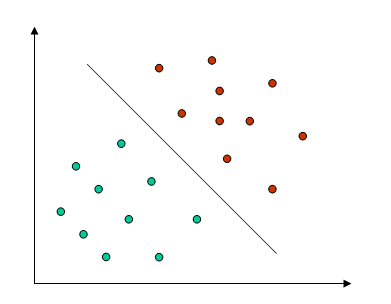
\includegraphics[width=70mm,scale=0.7]{LDA.png}
  \caption{Sehr grober Vorgang bei einem LDA. Die verschiedenfarbigen Punkte repräsentieren verschiedene Klassen. \cite{Wikimedia-Common3}}
  \label{fig:lda1}
\end{figure}

\subsection{KNN}
K-Nearest Neighbors arbeitet, indem es den Abstand von einem Testbeispiel zu den bekannten Werten eines Trainingsbeispiels berechnet. Die Gruppe von Datenpunkten, die den kleinsten Abstand zwischen den Trainingspunkten und dem Testpunkt ergeben, ist die ausgewählte Klasse. In der Abbildung  \ref{fig:knn1} sieht man Datenpunkte aus drei verschiedenen Klassen. In  \ref{fig:knn2} ist der Gebrauch eines KNN Algorithmus zu sehen. Man kann sehen, dass die meisten Datenpunkte, die Nachbarn waren, auch zur selben Klasse gehören. 

\begin{figure}[H]
  \centering
  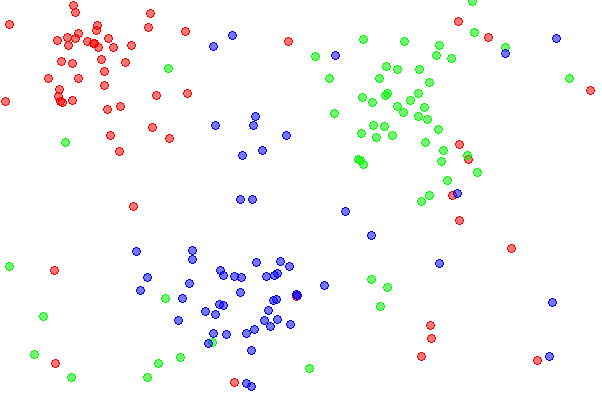
\includegraphics[width=70mm,scale=0.7]{KNN2.png}
  \caption{Datenpunkte von 3 Klassen. Die Klassen hier sind Rot, Grün und Blau.\cite{Wikimedia-Common2} }
  \label{fig:knn1}
\end{figure}

\begin{figure}[H]
  \centering
  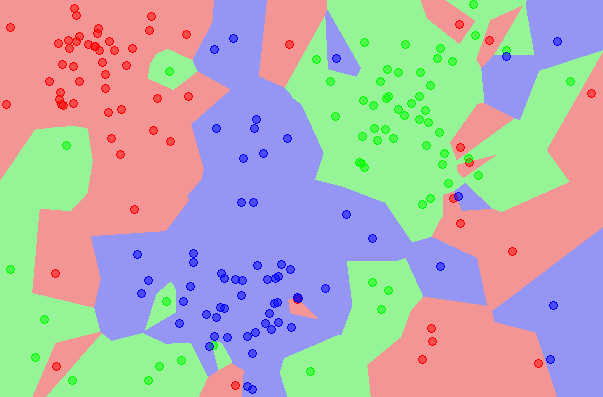
\includegraphics[width=70mm,scale=0.7]{KNN1.png}
  \caption{KNN angepasst an die Daten von \ref{fig:knn1}\cite{Wikimedia-Common} }
  \label{fig:knn2}
\end{figure}


\subsection{DecisionTree}
Ein DecisionTree-Klassifikator funktioniert, indem er einen Datensatz auf der Grundlage verschiedener Kriterien in immer kleinere Teilmengen zerlegt. Zur Unterteilung des Datensatzes werden verschiedene Sortierkriterien verwendet, wobei die Anzahl der Beispiele mit jeder Unterteilung kleiner wird.

Sobald das Netzwerk die Daten auf ein Beispiel herunter gebrochen hat, wird das Beispiel in eine Klasse eingeordnet. Wenn mehrere DecisionTree Klassifikatoren miteinander verknüpft werden, werden sie RandomForest-Klassifikator genannt.


\subsection{RandomForest}
Randomforest ist ein überwachter maschineller Lernalgorithmus, der auf Ensemble-Lernen basiert. Ensemble-Lernen ist eine Art des Lernens, bei dem man verschiedene Arten von Algorithmen oder denselben Algorithmus mehrfach miteinander verbindet, um ein besseres Vorhersagemodell zu bauen. Der RandomForest-Algorithmus kombiniert mehrere Entscheidungsbäume.
\clearpage

\subsection{SVC}
SVCs(Support Vector Machines) arbeiten, indem sie eine Linie zwischen den verschiedenen Clustern von Datenpunkten ziehen, um diese in Klassen zu gruppieren. Die Klassen werden dann je nach den Abständen der Punkte zu den Linien eingeteilt.

Die Abbildungen \ref{fig:svc1} und  \ref{fig:svc2} zeigen einen Datensatz vor und nach dem Trainieren eines oben erklärten SVC-Klassifikators. Es wird der Abstand der  Punkte zur gezeichneten Linie gemessen. Dadurch wird ermittelt, dass Blau  zu einer Klasse und Gelb  zu einer anderen Klasse gehört.



\begin{figure}[H]
  \centering
  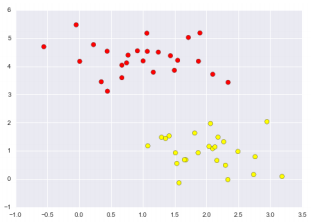
\includegraphics[width=70mm,scale=0.7]{SVC1.png}
  \caption{Daten für die Durchführung des SVC Algorithmus. Die gelben und blauen Punkte stehen für Datenpunkte verschiedener Klassen. Die Einheiten der Achsen sind unwichtig für die Darstellung. \cite{10.5555/3133359}}
  \label{fig:svc1}
\end{figure}

\begin{figure}[H]
  \centering
  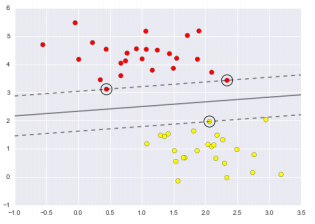
\includegraphics[width=70mm,scale=0.7]{SVC2.png}
  \caption{Ein SVM-Klassifikator, der an die Daten angepasst ist, mit Margins (gestrichelte
Linien) und den Stützvektoren (Kreise) dargestellt. Die Einheiten der Achsen sind unwichtig für die Darstellung. \cite{10.5555/3133359}} 
  \label{fig:svc2}
\end{figure}